\documentclass[a5paper,6pt]{article}
\usepackage[utf8]{inputenc}
\usepackage{lmodern}
\usepackage[MeX]{polski}
\usepackage{geometry}
\usepackage{fontspec}
\usepackage{fontawesome}
\usepackage{color}
\usepackage{adjustbox}
\usepackage[table]{xcolor}
\usepackage{tikz-qtree}
\usepackage{minted}
\usepackage{tcolorbox}
\usepackage{array,ragged2e,pst-node,pst-dbicons}

\usepackage{tikz}
\usetikzlibrary{shapes.multipart}
\usetikzlibrary{matrix}
\usetikzlibrary{positioning}
\usetikzlibrary{shadows}
\usetikzlibrary{calc}

\newcolumntype{C}[1]{>{\Centering}p{#1}}
\def\Tab#1{\tabular{C{3cm}}\rule[-5mm]{0pt}{1cm}#1\\\hline
                           ~\\\hline~\endtabular}
\seticonparams{entity}{shadow,fillcolor=black!20,fillstyle=solid,framesep=0pt}

\setmainfont[Color=primary, Path = fonts/lato/,
BoldItalicFont=Lato-RegIta,BoldFont=Lato-Reg,ItalicFont=Lato-LigIta]{Lato-Lig}
\setmonofont{Fira Code Light}

\colorlet{punct}{red!60!black}
\definecolor{background}{HTML}{EEEEEE}
\definecolor{delim}{RGB}{20,105,176}
\colorlet{numb}{magenta!60!black}

\newgeometry{tmargin=2cm, bmargin=2cm, lmargin=1.5cm, rmargin=1.5cm}
\setlength{\parindent}{0cm}

% \linespread{0.9}

\newcommand{\horrule}[1]{\rule{\linewidth}{#1}}
\newcommand\tab[1][1cm]{\hspace*{#1}}

\makeatletter
\pgfarrowsdeclare{crow's foot}{crow's foot}
{
  \pgfarrowsleftextend{+-.5\pgflinewidth}%
  \pgfarrowsrightextend{+.5\pgflinewidth}%
}
{
  \pgfutil@tempdima=0.5pt%
  \advance\pgfutil@tempdima by.25\pgflinewidth%
  \pgfsetdash{}{+0pt}%
  \pgfsetmiterjoin%
  \pgfpathmoveto{\pgfqpoint{0pt}{-6\pgfutil@tempdima}}%
  \pgfpathlineto{\pgfqpoint{-6\pgfutil@tempdima}{0pt}}%
  \pgfpathlineto{\pgfqpoint{0pt}{6\pgfutil@tempdima}}%
  \pgfusepathqstroke%
}


\tikzset{
    entity/.code={
        \tikzset{
            label=above:#1,
            name=#1,
            inner sep=0pt,
            every entity/.try,
            fill=white,
            general shadow={
                shadow xshift=0.0625in,
                shadow yshift=-0.0625in,
                opacity=0.5,
                fill=black!50
            }
        }%
        \def\entityname{#1}%
    },
    entity anchor/.style={matrix anchor=#1.center},
    every entity/.style={
            draw,
    },
    every property/.style={
        inner xsep=0.25cm, inner ysep=0.125cm, anchor=west, text width=1in
    },
    zig zag to/.style={
        to path={(\tikztostart) -| ($(\tikztostart)!#1!(\tikztotarget)$) |- (\tikztotarget)}
    },
    zig zag to/.default=0.5,
    one to many/.style={
        -crow's foot, zig zag to
    },
    many to one/.style={
        crow's foot-, zig zag to
    },
    many to many/.style={
        crow's foot-crow's foot, zig zag to
    }
}
\def\property#1{\node[name=\entityname-#1, every property/.try]{#1};}
\def\properties{\begingroup\catcode`\_=11\relax\processproperties}
\def\processproperties#1{\endgroup%
    \def\propertycode{}%
    \foreach \p in {#1}{%
        \expandafter\expandafter\expandafter\gdef\expandafter\expandafter\expandafter\propertycode%
            \expandafter\expandafter\expandafter{\expandafter\propertycode\expandafter\property\expandafter{\p}\\}%
    }%
    \propertycode%
}


% \title{Bazy Danych}
% \author{Pytania egzaminacyjne}

\title{%
  Bazy Danych \\
  \large Pytania egzaminacyjne}
\author{Hubert Jaremko}
\date{2018/2019}
\frenchspacing

\begin{document}
    \maketitle
    \tableofcontents
    \pagebreak

    \section{Architektury systemów baz danych} % (fold)
    \label{sec:architektury_systemow}

    % section architektury_systemów_baz_danych (end)

    \section{Relacyjny model danych, normalizacja relacji} % (fold)
    \label{sec:relacyjny_model_danych_normalizacja_relacji}

    \horrule{0.5pt}
    Proszę \underline{podać przykład} tabeli (relacji), która \textbf{jest w
    trzeciej} postaci normalnej, ale \textbf{nie jest} w postaci normalnej
    \textbf{Boyce’a Codd’a}.\\
    \horrule{0.5pt}\\

    Relacja \texttt{\{Miasto, Ulica, Kod\}}\\
    Klucze:
    \begin{enumerate}
        \item \texttt{\{Miasto, Ulica\}}
        \item \texttt{\{Ulica, Kod\}}
    \end{enumerate}

    Dodatkowe zależności:
    \begin{enumerate}
        \item \texttt{ \{Kod\} --> \{Miasto\}}\\
    \end{enumerate}

    \begin{tcolorbox}
    \textbf{Tylko 3NF} - \texttt{Kod} nie jest nadkluczem.
    \end{tcolorbox}


% \pagebreak

    \horrule{0.5pt}
    Dla tabeli (relacji) z podanymi zależnościami funkcyjnymi \underline{proszę
     powiedzieć} w której \textbf{postaci normalnej} jest ta tabela.\\
    \horrule{0.5pt}\\

    Relacja \texttt{\{CustomerID, Firstname, Surname, Telephone\}}\\
    Klucze: \texttt{\{CustomerID, Telephone\}}\\
    Dodatkowe zależności:
    \begin{enumerate}
        \item \texttt{ \{CustomerID\} --> \{Firstname, Surname\}}
        \item \texttt{ \{Telephone\} --> \{CustomerID\}}
    \end{enumerate}

    \begin{tcolorbox}
    \textbf{Tylko 1NF} - Częściowa funkcyjna zależność atrybutu wtórnego od
    podzbioru właściwego klucza w zależności nr 2.
    \end{tcolorbox}

\pagebreak

    Relacja \texttt{\{Tournament, Year, Winner, Winner Date of Birth\}}\\
    Klucze: \texttt{\{Tournament, Year\}}\\
    Dodatkowe zależności:
    \begin{enumerate}
        \item \texttt{ \{Winner\} --> \{Winner Date of Birth\}}
    \end{enumerate}

    \begin{tcolorbox}
    \textbf{Tylko 2NF} - Atrybut niekluczowy funkcyjnie zależny od innego
    atrybutu niekluczowego.
    \end{tcolorbox}

    \vskip 0.5cm
    Relacja \texttt{\{PESEL, NrPłyty, Od, Do, NrDowodu\}}\\
    Klucze:
    \begin{enumerate}
        \item \texttt{\{PESEL, NrPłyty, Od\}}
        \item \texttt{\{NrDowodu, NrPłyty, Od\}}
    \end{enumerate}

    Dodatkowe zależności:
    \begin{enumerate}
        \item \texttt{ \{NrDowodu\} --> \{PESEL\}}
    \end{enumerate}

    \begin{tcolorbox}
    \textbf{Tylko 3NF} - Lewa strona zależności nr 1 nie jest nadkluczem.
    \end{tcolorbox}

    \vskip 0.5cm
    Relacja \texttt{\{Restaurant, Pizza Type, Delivery Area\}}\\
    Klucze: \texttt{\{Restaurant, Pizza Type, Delivery Area\}}

    Dodatkowe zależności:
    \begin{enumerate}
        \item \texttt{ \{Restaurant\} ->> \{Pizza Type\}}
        \item \texttt{ \{Restaurant\} ->> \{Delivery Area\}}
    \end{enumerate}

    \begin{tcolorbox}
    \textbf{Tylko BCNF} - Jeśli założymy, że wszystkie typy pic są dowożone na
    każdy obszar to występują nietrywialne zależności wielowartościowe, których
    lewa strona nie zawiera klucza.
    \end{tcolorbox}

\pagebreak

    \horrule{0.5pt}
    Podaną tabelę należy doprowadzić do
    \textbf{postaci normalnej Boyce’a Codd’a}.\\
    \horrule{0.5pt}

    \vskip 0.5cm

    \textbf{PRZYKŁAD 1.}

    \vskip 0.5cm

\begin{adjustbox}{width=\columnwidth,center}
    % \begin{center}
    \begin{tabular}{|l|l|l|l|l|l|}
        \hline
        \textbf{Tytuł} &
        \textbf{Rok} &
        \textbf{Długość} &
        \textbf{TypFilmu} &
        \textbf{NazwaStudia} &
        \textbf{AdresStudia}\\
        \hline
        Gwiezdne Wojny &
        1977 &
        124 &
        kolor &
        Fox &
        Hollywood \\
        \hline
        Poteżne Kaczory &
        1991 &
        104 &
        kolor &
        Disney &
        Buena Vista \\
        \hline
        Świat Wayna &
        1992 &
        95 &
        kolor &
        Paramount &
        Hollywood \\
        \hline
        Rodzina Adamsów &
        1991 &
        102 &
        kolor &
        Paramount &
        Hollywood \\
        \hline
        \end{tabular}
    % \end{center}
\end{adjustbox}

    \vskip 0.5cm

    \textbf{Klucz:} \texttt{\{Tytuł, Rok\}}\\
    \textbf{Zależność funkcyjna:} \texttt{\{NazwaStudia\} --> \{AdresStudia\}}\\

    \textbf{Dekomponujemy schemat na dwa zbiory:}\\
    \texttt{\{\underline{NazwaStudia}, AdresStudia\}}\\
    \texttt{\{NazwaStudia, \underline{Tytuł, Rok}, Długość, TypFilmu\}}\\

    \vskip 0.5cm

    \textbf{PRZYKŁAD 2.}

    \vskip 0.5cm

% \begin{adjustbox}{width=\columnwidth,center}
    \begin{center}
    \begin{tabular}{|l|l|l|}
        \hline
        \textbf{Person} &
        \textbf{Shop Type} &
        \textbf{Nearest Shop}\\
        \hline
        Davidson & Optician & Eagle Eye \\
        \hline
        Davidson & Hairdresser & Snippets \\
        \hline
        Wright & Bookshop & Merlin Books \\
        \hline
        Fuller & Bakery & Doughy's \\
        \hline
        Fuller & Hairdresser & Sweeney Todd's \\
        \hline
        Fuller & Optician & Eagle Eye \\
        \hline
        \end{tabular}
    \end{center}
% \end{adjustbox}

    \vskip 0.5cm

    \textbf{Klucze:} \texttt{\{Person, Shop Type\}; \{Person, Nearest Shop\}}\\
    \textbf{Zależność funkcyjna:} \texttt{\{Nearest Shop\} --> \{Shop Type\}}\\

    \textbf{Dekomponujemy schemat na dwa zbiory:}\\
    \texttt{\{\underline{Nearest Shop}, Shop Type\}}\\
    \texttt{\{\underline{Nearest Shop, Person}\}}\\

\pagebreak

    \horrule{0.5pt}
    Proszę \underline{podać przykład} uzasadniający \textbf{denormalizację}.\\
    \horrule{0.5pt}\\

    \texttt{\textbf{Adresy:}\\
    \{\textbf{{\color{green}\faKey}NrPracownika}, Ulica, Miasto,
    Województwo, KodPocztowy\}}\\

    Zakładamy nastepujące zależności funkcyjne:
    \begin{enumerate}
        \item \texttt{\{Ulica, Miasto, Województwo\} --> \{KodPocztowy\}}
        \item \texttt{\{KodPocztowy\} --> \{Miasto, Województwo\}}
    \end{enumerate}

    Relacja \texttt{Adresy} jest w 2NF, ale nie jest w 3NF.\\

    \textbf{Rozwiązanie 1} (wynikające z zależności funkcyjnej 1.)\\

    \texttt{\{{\color{green}\faKey}{\color{blue}\faKey}Ulica,
    {\color{green}\faKey}Miasto, {\color{green}\faKey}Województwo,
    {\color{blue}\faKey}KodPocztowy\}} (*)\\
    \texttt{\{{\color{green}\faKey}NrPracownika, Ulica, Miasto, Województwo\}}
    (**)\\

    Relacja (*) jest w 3NF, ale nie jest BCNF.\\
    Relacja (**) jest w BCNF.\\

    Zostały zachowane zależności funkcyjne, ale jest redundancja.\\
    Tabele bedą \underline{łączone ze sobą aż przez \textbf{trzy} pola}
    (klucz obcy złożony).\\
    Można tego uniknąć poprzez dodanie atrybutu \texttt{ IdAdresu } do
    relacji (*) z zależnością funkcyjną \texttt{\{IdAdresu\} --> \{Ulica,
    Miasto, Województwo\}} oraz wstawienie \texttt{ IdAdresu } zamiast
    \texttt{\{Ulica, Miasto, Województwo\}} w relacji (*). Mielibyśmy:\\

    \texttt{\{{\color{red}\faKey}IdAdresu,
    {\color{green}\faKey}{\color{blue}\faKey}Ulica,
    {\color{green}\faKey}Miasto, {\color{green}\faKey}Województwo,
    {\color{green}\faKey}KodPocztowy\}}
    (tylko 3NF)\\
    \texttt{\{{\color{green}\faKey}NrPracownika, IdAdresu\}} (BCNF)\\

    Wróćmy jednak do rozwiązania bez \texttt{IdAdresu}. W pierwszej relacji jest
    redundancja. Można dekomponować pierwszą relacje na dwie, doprowadzają do
    BCNF:\\
    \texttt{\{Miasto, Województwo, {\color{blue}\faKey}KodPocztowy\}} oraz\\
    \texttt{\{{\color{green}\faKey}Ulica, {\color{green}\faKey}KodPocztowy\}}\\

    Ostatecznie otrzymamy trzy relacje:\\
    \texttt{\{Miasto, Województwo, {\color{blue}\faKey}KodPocztowy\}}\\
    \texttt{\{{\color{green}\faKey}Ulica, {\color{green}\faKey}KodPocztowy\}}\\
    \texttt{\{{\color{green}\faKey}NrPracownika, Ulica, Miasto, Województwo\}}\\

    \textbf{"Zgubiliśmy" zależność funkcyjną nr 1}. Ponadto uzyskanie kodu
    pocztowego\\ pracownika \underline{wymaga złączenia trzech tabel}.\\

    W przypadku wersji z atrybutem \texttt{ IdAdresu } otrzymalibyśmy:

    \texttt{\{Miasto, Województwo, {\color{blue}\faKey}KodPocztowy\}}\\
    \texttt{\{{\color{red}\faKey}IdAdresu, {\color{blue}\faKey}Ulica,
    {\color{blue}\faKey}KodPocztowy\}}\\
    \texttt{\{{\color{green}\faKey}NrPracownika, IdAdresu\}}\\

    "Zgubiliśmy" zależność funkcyjną nr 1. Uzyskanie miasta i województwa
    pracownika \underline{wymaga złączenia trzech tabel}.\\

    \textbf{Rozwiązanie 2} (wynikające z zależności funkcyjnej 1.)\\

    \texttt{\{{\color{green}\faKey}KodPocztowy, Miasto, Województwo\}}\\
    \texttt{\{{\color{green}\faKey}NrPracownika, Ulica, KodPocztowy\}}\\

    Obie relacje są w BCNF.\\
    Obydwie wcześniej przedstawione \textbf{zależności funkcyjne zostały
    "zgubione"}.
    Połączenie miedzy tabelami bedzie realizowane przez jedno pole.\\\\

    Obydwa rozwiązania mają swoje wady i zalety. Zalety i wady ma również
    wyjściowa relacja \texttt{Adresy} (chociaż jest tylko w 2NF, nie jest w
    3NF).

\pagebreak

    \horrule{0.5pt}
    Proszę \underline{podać przykład} tabeli, która jest w postaci normalnej
    \textbf{Boyce’a Codd’a}, a w której jest \textbf{redundancja}.\\
    \horrule{0.5pt}

    \vskip 0.5cm

% \begin{adjustbox}{width=\columnwidth,center}
    \begin{center}
    \begin{tabular}{|l|l|l|}
        \hline
        \textbf{Nr Pracownika} &
        \textbf{Język Programowania} &
        \textbf{Język Obcy}\\
        \hline
        1 & C & niemiecki \\
        \hline
        1 & Java & angielski \\
        \hline
        2 & C & francuski \\
        \hline
        2 & Java & niemiecki \\
        \hline
        2 &  & hiszpański \\
        \hline
        \end{tabular}
    \end{center}
% \end{adjustbox}

    \vskip 0.5cm

    \textbf{Klucz:}\texttt{\{Nr Pracownika, Język Programowania, Język Obcy\}}\\
    \textbf{Zależności:}
    \begin{enumerate}
        \item \texttt{\{Nr Pracownika\} ->> \{Język Programowania\}}
        \item \texttt{\{Nr Pracownika\} ->> \{Język Obcy\}}
    \end{enumerate}

    \begin{tcolorbox}
    \textbf{Tylko BCNF} - Występują zależności wielowartościowe, których lewa
    strona nie zawiera klucza.
    \end{tcolorbox}

% \pagebreak

    \horrule{0.5pt}
    Proszę \underline{podać przykład} tabeli, która jest w \textbf{5NF},
    ale jest w niej \textbf{redundancja}.\\
    \horrule{0.5pt}

    \vskip 0.5cm

% \begin{adjustbox}{width=\columnwidth,center}
    \begin{center}
    \begin{tabular}{|l|l|l|}
        \hline
        \textbf{Producent} &
        \textbf{Wyrób} &
        \textbf{Część}\\
        \hline
        1 & 1 & 1 \\
        \hline
        1 & 2 & 1 \\
        \hline
        \end{tabular}
    \end{center}
% \end{adjustbox}

    \vskip 0.5cm

    \textbf{Klucz:} \texttt{\{Producent, Wyrób, Część\}}\\

    \begin{tcolorbox}
    \textbf{5CNF} - Zakładamy, że \texttt{Producent} może produkować daną część
    tylko do jednego wyrobu, nawet jeśli mogłaby być użyta w innym. Zatem
    \textbf{brak zależności wielowartościowych oraz klucz obejmuje wszystkie
    atrybuty} a wciąż jest redundancja (powtarzamy, że \texttt{Producent} 1
    produkuje \texttt{Część} 1).
    \end{tcolorbox}

\pagebreak

    \horrule{0.5pt}
    Proszę \underline{przedstawić} algorytm doprowadzenia relacji do
    \textbf{postaci normalnej Boyce’a Codd’a}.\\
    \horrule{0.5pt}

    \begin{itemize}
        \item Szukamy wszystkich \underline{nietrywialnych, pełnych zależności
              funkcyjnych}, które naruszają warunek BCNF, tzn.
              \textbf{lewa strona} zalezności funkcyjnej
              \textbf{nie jest nadkluczem}.
        \item Bierzemy jedną z takich zależności funkcyjnych $A \rightarrow B$
              (obojetnie którą, algorym jest niederministyczny).
        \item Dzielimy schemat relacji na dwa nierozłączne podzbiory:
              jeden zawierający wszystkie atrybuty wystepujące w zależności (*)
              naruszającej BCNF,
              drugi zawierający atrybuty z lewej strony rozważanej zależności
              (*) oraz atrybuty nie wystąpujące ani z lewej ani z prawej strony
              tej zależności.
        \item Strategie stosujemy do relacji powstałych w wyniku dekompozycji
              do chwili, gdy wszystkie relacje są w BCNF.
    \end{itemize}

    % section relacyjny_model_danych_normalizacja_relacji (end)

\pagebreak

    \section{Model ER} % (fold)
    \label{sec:model_er}

    \horrule{0.5pt}
    Proszę \underline{przedstawić przykład} diagramu \textbf{ER} w notacji
    \textbf{Barkera}, zawierającego dwie encje i związek między nimi (związek
    bez własnych atrybutów). Diagram powinien być taki, że po jego
    transformacji do modelu relacyjnego \textbf{otrzymamy trzy relacje} (trzy
    tabele).\\
    \horrule{0.5pt}

    % \includegraphics[scale=0.521]{erd}

\begin{center}
\begin{tikzpicture}[node distance=1.25in]

\matrix [entity=Pracownik] {
    \properties{
        +IdPracownika,
        *Nazwisko,
        *Etat,
        *Pensja
    }
};

\matrix [entity=Projekt, right=of Pracownik-+IdPracownika, entity anchor=Projekt-+NrProjektu]  {
    \properties{
        +NrProjektu,
        *Nazwa,
        *Sponsor
    }
};

\draw [many to many] (Pracownik-+IdPracownika)   to (Projekt-+NrProjektu);
\end{tikzpicture}
\end{center}

% \vskip 0.1cm

    % \begin{center}
    % \entity{pracownik}[
    %     \begin{tabular}{l}
    %       Pracownik \\
    %       \hline
    %       \#~IdPracownika \\
    %       \textasteriskcentered~Nazwisko \\
    %       \textasteriskcentered~Etat \\
    %       \textasteriskcentered~Pensja \\
    %     \end{tabular}
    % ]\hspace{2.5cm}
    % \entity{projekt}[
    %     \begin{tabular}{l}
    %       Projekt \\
    %       \hline
    %       \#~NrProjektu \\
    %       \textasteriskcentered~Nazwa \\
    %       \textasteriskcentered~Sponsor \\
    %     \end{tabular}
    % ]
    % \ncline[arrowscale=2]{>-<}{pracownik}{projekt}
    % \naput[npos=0.1]{M}\naput[npos=0.85]{N}
    % \end{center}

    Po transformacji diagramu zostaną utworzone trzy tabele.
    \begin{center}
    \begin{tabular}{cc}
        \begin{minipage}{.5\linewidth}

        \begin{center}
            \begin{tabular}{|l|}
              \hline
              \texttt{Pracownicy} \\
              \hline
              \texttt{\#~IdPracownika} \\
              \texttt{*~Nazwisko} \\
              \texttt{*~Etat} \\
              \texttt{*~Pensja} \\
              \hline
            \end{tabular}
        \end{center}

        \end{minipage} &
        \begin{minipage}{.5\linewidth}

        % \begin{center}
            \begin{tabular}{|l|}
              \hline
              \texttt{Projekty} \\
              \hline
              \texttt{\#~NrProjektu} \\
              \texttt{*~Nazwa} \\
              \texttt{*~Sponsor} \\
              \hline
            \end{tabular}
        % \end{center}

        \end{minipage}
    \end{tabular}
    \end{center}

    \begin{center}
    \begin{tabular}{|l|}
      \hline
      \texttt{Pracownicy\_Projekty} \\
      \hline
      \texttt{\#~IdPracownika REFERENCES Pracownicy(IdPracownika)} \\
      \texttt{\#~NrProjektu REFERENCES Projekty(NrProjektu)} \\
      \texttt{PRIMARY KEY (IdPracownika, NrProjektu)}\\
      \hline
    \end{tabular}
    \end{center}

    \horrule{0.5pt}
    Proszę \underline{omówić} trzy schematy \textbf{transformacji hierarchii}
    encji do modelu relacyjnego.\\
    \horrule{0.5pt}

    \begin{enumerate}
        \item Utworzenie \textbf{jednej tabeli ze wszystkimi} atrybutami i
              kluczami obcymi, tj. wspólnymi i specyficznymi dla podencji.
        \item Utworzenie \textbf{osobej tabeli dla każdej podencji}.
        \item Utworzenie \textbf{osobnej tabeli na atrybuty wspólne i osobnej
              tabeli dla każdej podencji}.\\
              Tabele powstałe z podencji zawierają klucz podstawiowy i atrybuty
              specyficzne, tabela wspólna i tabele powstałe z podencji są
              połączone ograniczeniami referencyjnymi.
    \end{enumerate}

    % section model_er (end)

    \section{Transakcje} % (fold)
    \label{sec:transakcje}

    \subsection{Właściwiości (ACID)} % (fold)
    \label{sub:wlasciwiosci}

    \horrule{0.5pt}
     Proszę omówić własności \textbf{ACID} transakcji. W jaki sposób
          implementowane są własności \textbf{A i D}? Proszę podać jak
          wykorzystywany jest \textbf{dziennik transakcji} oraz co to jest
          strategia \textbf{No-Fix/No-Flush} i jak wpływa ona na sposoby
          odtwarzania systemu po awarii.\\
    \horrule{0.5pt}

    \textbf{WŁASNOŚCI ACID}
    \begin{itemize}
        \item \textbf{Atomicity} \textit{(atomowość, niepodzielność)}
        \begin{itemize}
            \item Transakcja jest niepodzielną jednostką przetwarzania, musi
                  być wykonywana w całości lub wcale.
        \end{itemize}

        \item \textbf{Consistency} \textit{(spójność)}
        \begin{itemize}
            \item Po wykonaniu transakcji baza danych musi być w stanie spójnym,
                  tj. muszą zostać zachowane wszystkie więzy narzucone na dane.
        \end{itemize}

        \item \textbf{Isolation} \textit{(separacja, izolacja)}
        \begin{itemize}
            \item Transakcja powinna wyglądać tak, jakby była wykonywana w
                  izolacji od innych transakcji.
        \end{itemize}

        \item \textbf{Durability} \textit{(trwałość)}
        \begin{itemize}
            \item Po zatwierdzeniu transakcji jej efekty muszą być trwałe w
                  systemie, nawet jeśli nastąpi uszkodzenie systemu natychmiast
                  po zatwierdzeniu.
        \end{itemize}

    \end{itemize}

    \textbf{IMPLEMENTACJA A I D}
    \begin{itemize}
        \item Za odtwarzanie i w pewnym sensie za \textbf{atomowość, trwałość}
              oraz spójność, jest odpowiedzialny \textbf{moduł zarządzania
              odtwarzaniem} \textit{(recovery-management component).}

        \item Modyfikacja danych następuje w buforze w pamięci RAM. Buforem
              zarządza specjalny menadżer \textit{(zarządca)}.
              W pewnym momencie zarządca bufora musi skopiować nową zawartość
              bloku z powrotem na dysk.
    \end{itemize}

\pagebreak

    \textbf{STRATEGIA NO-FIX/NO-FLUSH}
    \begin{itemize}
        \item Stosowana w większości relacyjnych systemów baz zdanych
              wykorzystujących dzienniki transakcji.

        \item \textbf{NO-FIX}
        \begin{itemize}
            \item Blok skopiowany do RAM \textbf{może} być skopiowany lub
                  przeniesiony z powrotem na dysk zanim transakcja, która ten
                  blok zmodyfikowała się skończy.
        \end{itemize}

        \item \textbf{NO-FLUSH}
        \begin{itemize}
            \item Na końcu transakcji \textbf{nie ma obowiązku}
                  zsynchronizowania zmienionych przez tę transakcję bloków
                  z dyskiem.
            \item Synchronizacja może być wykonana później.
            \item \underline{Zwiększa wydajność}.
            \item Na tradycyjnych dyskach HDD operacje kopiowania bloków mogą
                  być grupowane.
        \end{itemize}
    \end{itemize}

    \textbf{WPŁYW NA SPOSOBY ODTWARZANIA SYSTEMU PO AWARII}
    \begin{itemize}
        \item \textbf{No-Flush} oznacza, że nie mamy gwarancji, że natychmiast
              po zakończeniu transakcji na dysku znajdą się zmienione dane.
        \item Trwałość transakcji w większości systemów zapewniają
              \textbf{dzienniki transakcji}.
        \item \textbf{No-Fix} oznacza, że może się zdarzyć, że blok zmieniony
              przez transakcje zostanie skopiowany na dysk, zanim transakcja
              zakończy się.
        \item Synchronizacja buforów z RAM z dyskiem może być realizowane
              cyklicznie w ramach \textbf{punktów kontrolnych}
              \textit{(control point, check point)}.
        \item \textbf{Punkty kontrolne} ułatwiają \textbf{odtwarzanie systemu
              po awarii}, kiedy dyski z danymi i z dziennikiem transakcji nie
              zostały uszkodzone.

    \pagebreak

        \item \textbf{Odtwarzanie po awarii systemu (RECOVERY)}
        \begin{itemize}
            \item redo
            \item undo
        \end{itemize}

        \item \textbf{Odtwarzanie po awarii dysków z danymi}
        \begin{itemize}
            \item RESTORE \textit{(przywracanie plików z kopii zapasowych)}
            \item RECOVERY
        \end{itemize}
    \end{itemize}

    \textbf{STOSOWANIE DZIENNIKA TRANSAKCJI}
    \begin{itemize}
        \item \textbf{Dziennik transakcji} jest plikiem na dysku, zawierającym
              \textbf{informację o\\ wszystkich wprowadzonych} przez transakcję
              \textbf{zmianach}.
        \item Transakcja \textbf{nie jest uznana} za zakończoną, jeśli fizycznie
              na dysku w pliku dziennika nie znajdą się \textbf{wpisy opisujące
              \underline{wszystkie} zmiany} oraz \textbf{informacja o
              zatwierdzeniu} transakcji.
        \item Wpis (rekord) w dzienniku może zawierać znacznik transakcji, starą
              i nową wartość zmienianego elementu, informację o rodzaju
              operacji, może zawierać informację o tzw. operacji kompensującej.
              Są też wpisy dotyczące rozpoczęcia transakcji i jej
              zatwierdzenia, w pewnych systemach także wpisy dotyczące operacji
              odczytu.
        \item Dzięki dziennikowi można powtórzyć te operacje, których efekty nie
              zostały jeszcze zapisane na dysku, mimo że operacja została
              zatwierdzona (no-flush).
        \item \textbf{W przypadku odtwarzania po awarii} może być wymagane
              \textbf{powtórzenie} \textit{(redo)} niektórych operacji
              (zatwierdzone, ze względu na \textit{\textbf{No-Flush}} mogły\\
              jeszcze nie zostać zapisane) i \textbf{wycofanie} \textit{(undo)}
              innych (niezatwierdzone, ze względu na \textit{\textbf{No-Fix}}
              mogły już się zapisać).
    \end{itemize}

    % subsection właściwiości (end)

\pagebreak

    \subsection{Harmonogramy, szeregowalność konfliktowa i perspektywiczna}
    \label{sub:harmonogramy_szeregowalnosc_konfliktowa_i_perspektywiczna}

    \horrule{0.5pt}
    Proszę podać definicje \textbf{harmonogramu szeregowalnego, szeregowalnego
    konfliktowo i szeregowalnego perspektywicznie}. Jakie znaczenie w praktyce
    ma pojęcie \textbf{szeregowalności konfliktowej?}\\
    \horrule{0.5pt}

    \vskip 0.5cm

    \textbf{HARMONOGRAM SZEREGOWALNY}
    \begin{itemize}
        \item \textbf{Jeśli jego wpływ na stan bazy danych jest taki sam jak
              pewnego harmonogramu szeregowego, niezależnie od stanu
              początkowego tej bazy danych}.
        \item Harmonogramy są \textbf{równoważne co do wyniku}
              \textit{(result equivalent)}, jeżeli dają ten sam stan bazy danych
              bez względu na początkowy stan bazy.
    \end{itemize}

    \textbf{HARMONOGRAM SZEREGOWALNY KONFLIKTOWO}
    \textit{(conflict serializable)}
    \begin{itemize}
        \item Harmonogramy są \textbf{równoważne konfliktowo}
              \textit{(conflict equivalent)} jeżeli kolejność wszystkich
              operacji konfliktowych jest w nich taka sama.
        \item Dwie operacje są w stanie \textbf{konfliktu}, jeśli:
        \begin{itemize}
            \item Należą do różnych transakcji.
            \item Uzyskują dostep do tego samego elementu.
            \item Przynajmnej jedna z nich jest operacją zapisu.
        \end{itemize}

        \item Harmonogram \textbf{S} jest \underline{szeregowalny konfliktowo},
        jeżeli jest on \underline{równoważny} \underline{konfliktowo} z pewnym
        szeregowym harmonogramem \textbf{S'}.
        \item W takim przypadku możemy zamieniać kolejność niekonfliktowych
        operacji w \textbf{S} do momentu, aż utworzony zostanie równoważny
        harmonogram szeregowy \textbf{S'}.
    \end{itemize}

\pagebreak

    \textbf{HARMONOGRAM SZEREGOWALNY PERSPEKTYWICZNIE}\\
    \textit{(view serializability)}
    \begin{itemize}
        \item Jest on \textbf{równoważny perspektywicznie} pewnemu
        harmonogramowi szeregowemu.
        \item \textbf{Równoważność perspektywiczna}:
        \begin{itemize}
            \item Harmonogram \textbf{S i S'} zwierają te same instrukcje i dla
                  każdego elementu danych \textbf{Q}:
        \end{itemize}

\begin{adjustbox}{width=\columnwidth,center}
    \begin{tabular}{|l|l|}
        \hline
        $S$ & $S'$ \\
        \hline
        $T_k$ jest pierwszą transakcją, która czyta \textbf{Q} &
        $T_k$ musi być pierwszą transakcją, która czyta \textbf{Q} \\

        $T_i$ czyta \textbf{Q} zapisany przez $T_j$ &
        $T_i$ czyta \textbf{Q} zapisany przez $T_j$\\

        $T_m$ jest ostatnią transakcją, która zapisuje \textbf{Q} &
        $T_m$ jest ostatnią transakcją, która zapisuje \textbf{Q}\\
        \hline
    \end{tabular}
\end{adjustbox}

        \item Oznacza to samo co \textbf{szeregowalność konfliktowa, jeśli}
              założymy ograniczenie co do operacji \textbf{zapisów} we
              wszystkich transakcjach harmonogramu.
        \begin{itemize}
            \item Każda operacja \texttt{WRITE[x]} jest poprzedzona operacją
                  \texttt{READ[x]}
            \item Wartość zapisana przez \texttt{WRITE[x]} zależy tylko od
                  wartości elementu \texttt{x} odczytanej przez operacje
                  \texttt{READ[x]} (jest pewną nie stałą funkcją tylko elementu
                  \texttt{x}, nie zależy od wartości innych elementów.)
        \end{itemize}

        \item Szeregowalność perspektywiczna zapenia \textbf{spójność} bazy
              danych, ponieważ powoduje, że wyniki harmonogramu są takie same
              jak wyniki pewnego harmonogamu szeregowego.
    \end{itemize}

    \textbf{ZNACZENIE W PRAKTYCE SZEREGOWALNOŚCI KONFLIKTOWEJ}
    \begin{itemize}
        \item Zapewnia \textbf{spójność} bazy danych.
    \end{itemize}

\pagebreak

    \horrule{0.5pt}
    Proszę \underline{podać przykłady} harmonogramów \textbf{szeregowalnych}
    \underline{nie szeregowych}.\\
    \horrule{0.5pt}

    \begin{center}
    \begin{tabular}{|p{4cm}|p{4cm}|}
        \hline
        \textbf{$T_1$} & \textbf{$T_2$} \\
        \hline
        \texttt{read(A)} & \texttt{}\\
        \texttt{A := A - 50} & \texttt{}\\
        \texttt{write(A)} & \texttt{}\\
        \texttt{} & \texttt{read(A)}\\
        \texttt{} & \texttt{temp := A * 0.1}\\
        \texttt{} & \texttt{A := A - temp}\\
        \texttt{} & \texttt{write(A)}\\
        \texttt{read(B)} & \texttt{}\\
        \texttt{B := B + 50} & \texttt{}\\
        \texttt{write(B)} & \texttt{}\\
        \texttt{} & \texttt{read(B)}\\
        \texttt{} & \texttt{B := B + temp}\\
        \texttt{} & \texttt{write(B)}\\
        \hline
    \end{tabular}
    \end{center}

\pagebreak

    \horrule{0.5pt}
    Proszę \underline{podać przykłady} harmonogramów
    \textbf{szeregowalnych konfliktowo} i takich, które \textbf{nie są}
    szeregowalne konfliktowo.\\
    \horrule{0.5pt}

    \textbf{HARMONOGRAMY SZERGOWALNE KONFLIKTOWO}

    \begin{center}
    \begin{tabular}{|p{4cm}|p{4cm}|}
        \hline
        \textbf{$T_1$} & \textbf{$T_2$} \\
        \hline
        \texttt{read(A)} & \texttt{}\\
        \texttt{write(A)} & \texttt{}\\
        \texttt{} & \texttt{read(A)}\\
        \texttt{} & \texttt{write(A)}\\
        \texttt{read(B)} & \texttt{}\\
        \texttt{write(B)} & \texttt{}\\
        \texttt{} & \texttt{read(B)}\\
        \texttt{} & \texttt{write(B)}\\
        \hline
    \end{tabular}
    \end{center}

    \textbf{HARMONOGRAMY \underline{NIE}SZERGOWALNE KONFLIKTOWO}

    \begin{center}
    \begin{tabular}{|p{4cm}|p{4cm}|}
        \hline
        \textbf{$T_1$} & \textbf{$T_2$} \\
        \hline
        \texttt{read(A)} & \texttt{}\\
        \texttt{A := A - 50} & \texttt{}\\
        \texttt{write(A)} & \texttt{}\\
        \texttt{} & \texttt{read(B)}\\
        \texttt{} & \texttt{B := 5 - 10}\\
        \texttt{} & \texttt{write(B)}\\
        \texttt{read(B)} & \texttt{}\\
        \texttt{B := 5 + 50} & \texttt{}\\
        \texttt{write(B)} & \texttt{}\\
        \texttt{} & \texttt{read(A)}\\
        \texttt{} & \texttt{A := A + 10}\\
        \texttt{} & \texttt{write(A)}\\
        \hline
    \end{tabular}
    \end{center}

\pagebreak

    % subsection harmonogramy_szeregowalność_konfliktowa_i_perspektywiczna (end)

    \subsection{Poziomy izolacji transakcji} % (fold)
    \label{sub:poziomy_izolacji_transakcji}

    \horrule{0.5pt}
    Proszę \underline{omówić} \textbf{poziom izolacji} transakcji wybrany przez
    egzaminatora.\\
    \horrule{0.5pt}

    \vskip 1cm

% \begin{table}
\begin{adjustbox}{width=\columnwidth,center}
    % \begin{center}
    \begin{tabular}{|p{3cm}|p{1cm}|p{1cm}|p{2cm}|p{1cm}|p{1.3cm}|p{1.3cm}|}
      \hline
      \textbf{Poziom izolacji} &
      \textbf{P0 Dirty Write} &
      \textbf{P1 Dirty Read} &
      \textbf{P2 \newline Non-repeatable read} &
      \textbf{P3 Phantoms} &
      \textbf{Blokady X} &
      \textbf{Blokady S}\\
      \hline
      Locking READ \newline UNCOMMITTED &
      \cellcolor{red!25} NIE   &
      \cellcolor{green!25} TAK &
      \cellcolor{green!25} TAK &
      \cellcolor{green!25} TAK &
      \cellcolor{yellow!25} TAK, długie &
      Nie ma\\
      \hline
      Locking READ \newline COMMITTED &
      \cellcolor{red!25} NIE   &
      \cellcolor{red!25} NIE   &
      \cellcolor{green!25} TAK &
      \cellcolor{green!25} TAK &
      \cellcolor{yellow!25} TAK, długie &
      \cellcolor{cyan!15} TAK, krótkie\\
      \hline
      Locking REPEATABLE READ  &
      \cellcolor{red!25} NIE   &
      \cellcolor{red!25} NIE   &
      \cellcolor{red!25} NIE   &
      \cellcolor{green!25} TAK &
      \cellcolor{yellow!25} TAK, długie &
      \cellcolor{yellow!25} TAK, długie\\
      \hline
      Locking \newline SERIALIZABLE &
      \cellcolor{red!25} NIE &
      \cellcolor{red!25} NIE &
      \cellcolor{red!25} NIE &
      \cellcolor{red!25} NIE &
      \cellcolor{yellow!25} TAK, długie &
      \cellcolor{blue!25} TAK, długie, predykatowe\\
      \hline

    \end{tabular}
    % \end{center}
\end{adjustbox}
% \end{table}
    \vskip 1cm

    % \textbf{BLOKADY} \\
    \textbf{CURSOR STABILITY}
    \begin{itemize}
        \item READ COMMITTED « Cursor Stability « REPEATABLE READ
        \item Pewne rozszerzenie Locking READ COMMITTED.
        \item Dodaje sie operacje \texttt{READ\_CURSOR}
              \textit{(pobierz wiersz)} dla instrukcji \texttt{FETCH}.
        \item Blokada (\texttt{S} lub nowy typ do odczytu \textit{scroll lock})
              bedzie utrzymywana do\\ chwili przejścia do innego wiersza lub
              zamknięcia kursora.
        \item Aktualizacja wiersza przez kursor - operacja
              \texttt{WRITE\_CURSOR} powoduje\\ założenie na ten wiersz
              \textbf{blokady \texttt{X}} utrzymywanej do końca transakcji.
        \item \textbf{Eliminuje problem P4C}.
    \end{itemize}

    \textbf{SNAPSHOT ISOLATION} \textit{(First-commiter-wins)}
    \begin{itemize}
        \item Transakcja czyta dane (zatwierdzone) z chwili swojego początku,\\
              \textit{Start-Timestamp}.
        \item Wszelkie zmiany wykonywane są na lokalnych kopiach i zapisywane
              na końcu transakcji.
        \item Aktualizacje wykonywane przez inne transakcje nie są odczytywane.
        \item Jeśli $T_1$ jest gotowa do zatwierdzenia, otrzymuje
              \textit{Commit-Timestamp($T_1$)}, większy od wszystkich znaczników
              \textit{Start-Timestamp} i \textit{Commit-Timestamp}\\
              rozpoczętych i zakończonych już transakcji.
        \item Transakcja zostaje zatwierdzona tylko wówczas, jeśli żadna inna
              $T_2$
              z czasem zakończenia \textit{Commit-Timestamp($T_2$)} zawartym w
              przedziale\\
              \lbrack\textit{Start-Timestamp($T_1$)},~
              \textit{Commit-Timestamp($T_1$)}\rbrack~~nie zapisała danych,
              które zapisała również $T_1$.
        \item W przeciwnym wypadku $T_1$ zostaje wycofana.
        \item \textbf{\textit{First-commiter-wins} zapobiega lost update (P4).}
        \item Po zatwierdzeniu $T_1$, zmiany wykonane przez nią są widoczne
              przez wszystkie inne transakcje o czasie rozpoczecia wiekszym od
              \textit{Commit-Timestamp} transakcji $T_1$.
    \end{itemize}

    \textbf{SNAPSHOT ISOLATION} \textit{(First-writer-wins)}
    \begin{itemize}
        \item Podobnie jak wcześniej, ale są stosowane
              \textbf{blokady do zapisu}.
        \item Przy każdym zapisie transakcja wykonuje podobne sprawdzenie jak
              \textit{First-commiter-wins} na końcu transakcji.
        \item Przechowywane są różne wersje danych.
        \item Transakcja czyta dane zatwierdzone przed początkiem transakcji.
        \item \textbf{Brak blokad do odczytu}, operacja odczytu nie blokuje
              zapisu ani innych operacji odczytu.
        \item \textbf{Długotrwałe blokady wyłącznie do zapisu}.
        \item $T_1$ przy każdym zapisie sprawdza, czy istnieje $T_2$, która
              zmodyfikowała dane zapisywane i zakończyła sie powodzeniem.
        \item Jeśli tak, $T_1$ jest wycofywana.
        \item W systemie MS SQL Server tak działa poziom SNAPSHOT.
    \end{itemize}

    % subsection poziomy_izolacji_transakcji (end)
\pagebreak

    \subsection{Sterowanie współbieżnymi transakcjami w oparciu o blokady}
    \label{sub:sterowanie_wspolbieznymi_blokady}

    % subsection sterowanie_współbieżnymi_transakcjami_w_oparciu_o_blokady (end)

    \subsection{Sterowanie współbieżnymi transakcjami z wykorzystaniem
    wielowersyjności i blokad} % (fold)
    \label{sub:sterowanie_wspolbieznymi_wielowier}

    \horrule{0.5pt}
    Dla przedstawionego harmonogramu proszę podać jak będzie wyglądać sterowanie
    współbieżnością w wybranym przez egzaminatora poziomie izolacji
    transakcji.\\
    \horrule{0.5pt}

\pagebreak

    \horrule{0.5pt}
    Proszę \underline{omówić} wybrane przez egzaminatora \textbf{problemy}
    związane ze współbieżnym wykonaniem transakcji.\\
    \horrule{0.5pt}

    \textbf{P0 Dirty Write} \textit{(nadpisanie brudnopisu)}
    \begin{itemize}
        \item Transakcja $T_1$ modyfikuje daną.
        \item Transakcja $T_2$ dalej modyfikuje daną \textbf{zanim} $T_1$
              zostanie \textbf{zatwierdzona lub wycofana}.
        \item \texttt{WRITE\_1[x]}
        \item \texttt{WRITE\_2[x]}
        \item (\texttt{COMMIT\_1[x]} lub \texttt{ABORT\_1[x]}) i
              (\texttt{COMMIT\_2[x]} lub \texttt{ABORT\_2[x]})
              w dowolnej kolejności.
    \end{itemize}

    \textbf{P1 Dirty Read} \textit{(czytanie brudnopisu)}
    \begin{itemize}
        \item Transakcja $T_1$ modyfikuje daną.
        \item Transakcja $T_2$ czyta daną \textbf{zanim} $T_1$ zostanie
              zatwierdzona lub wycofana.
        \item \textbf{Jeśli} $T_1$ zostaje \textbf{wycofana} $T_2$ przeczytało
              daną, która nie została zatwierdzona czyli w sumie nigdy nie
              istniała.
        \item \texttt{WRITE\_1[x]}
        \item \texttt{READ\_2[x]}
        \item (\texttt{COMMIT\_1[x]} lub \texttt{ABORT\_1[x]}) i
              (\texttt{COMMIT\_2[x]} lub \texttt{ABORT\_2[x]})
              w dowolnej kolejności.
    \end{itemize}

    \textbf{P2 Non-repeatable read}
    \begin{itemize}
        \item Transakcja $T_1$ czyta daną.
        \item Transakcja $T_2$ modyfikuje lub usuwa daną oraz zostaje
              \textbf{zatwierdzona}.
        \item Jeśli $T_1$ spróbuje znowu przeczytać daną, otrzyma zmodyfikowaną
              wartość albo odkryje, że dana została skasowana.
        \item \texttt{READ\_1[x]}
        \item \texttt{WRITE\_2[x]}
        \item (\texttt{COMMIT\_1[x]} lub \texttt{ABORT\_1[x]}) i
              (\texttt{COMMIT\_2[x]} lub \texttt{ABORT\_2[x]})
              w dowolnej kolejności.
    \end{itemize}

    \textbf{P3 Phantoms}
    \begin{itemize}
        \item Transakcja $T_1$ czyta zestaw danych spełniający jakiś
              \textit{predykat}.
        \item Transakcja $T_2$ \textbf{tworzy daną} spełniająca ten
              \textit{predykat} i zostaje zatwierdzona.
        \item Jeśli $T_1$ spróbuje znowu przeczytać zestaw danych z tym samym\\
              \textit{predykat}em otrzyma zestaw danych
              \textbf{inny od pierwotnego}.
        \item \texttt{READ\_1[P]}
        \item \texttt{WRITE\_2[y in P]}
        \item (\texttt{COMMIT\_1[x]} lub \texttt{ABORT\_1[x]}) i
              (\texttt{COMMIT\_2[x]} lub \texttt{ABORT\_2[x]})
              w dowolnej kolejności.
    \end{itemize}

    \textbf{P4 Lost Update}
    \begin{itemize}
        \item Transakcja $T_1$ czyta element danych.
        \item Transakcja $T_2$ aktualizuje ten element i
              \textbf{zostaje zatwierdzona}.
        \item Transakcja $T_1$ aktualizuje ten sam element i
              \textbf{zostaje zatwierdzona}.
        \item \texttt{READ\_1[x]}
        \item \texttt{WRITE\_2[x]}
        \item \texttt{COMMIT\_2}
        \item \texttt{WRITE\_1[x]}
        \item \texttt{COMMIT\_1}
    \end{itemize}

    \textbf{P4C Lost Update} \textit{(dla operacji na kursorze)}
    \begin{itemize}
        \item \texttt{READ\_CURSOR\_1[x]}
        \item \texttt{WRITE\_2[x]}
        \item \texttt{COMMIT\_2}
        \item \texttt{WRITE\_CURSOR\_1[x]}
        \item \texttt{COMMIT\_1}
    \end{itemize}

    \textbf{A5A Read Skew} \textit{(skrzywiony odczyt)}
    \begin{itemize}
        \item Transakcja $T_1$ odczytuje \texttt{x}.
        \item Transakcja $T_2$ aktualizuje \texttt{x} oraz \texttt{y} i zostaje
              \textbf{zatwierdzona}.
        \item Jeśli $T_1$ odczyta \texttt{y} to będzie miała niespójny obraz
              danych.
        \item \texttt{READ\_1[x]}
        \item \texttt{WRITE\_2[x]}
        \item \texttt{WRITE\_2[y]}
        \item \texttt{COMMIT\_2}
        \item \texttt{READ\_1[y]}
        \item (\texttt{COMMIT\_1} lub \texttt{ABORT\_1})
    \end{itemize}


    \textbf{A5B Write Skew} \textit{(skrzywiony zapis)}\\\\
    Załóżmy, że na elementy danych \texttt{x} oraz \texttt{y} narzucono pewne
    ograniczenie \texttt{C()}. Każda transakcja z osobna dba o spełnienie
    \texttt{C()}.
    \begin{itemize}
        \item Transakcja $T_1$ odczytuje \texttt{x} (ew. też \texttt{y}).
        \item Transakcja $T_2$ odczytuje \texttt{y} (ew. też \texttt{x}).
        \item $T_1$ zapisuje \texttt{y} a $T_2$ zapisuje \texttt{x} i
              \textbf{obydwie zostają zatwierdzone}.
        \item Ostatnie cztery operacje mogą być zrealizowane w dowolnej
              (sensownej) kolejności.
        \item Każda transakcja przy zapisnie dba o spełnienie ograniczenia
              \texttt{C()}, jednak w wyniku przeplatanego wykonania ograniczenie
              \texttt{C()} może nie być spełnione po zatwierdzeniu obydwu
              transakcji.
        \item \texttt{READ\_1[x]}
        \item \texttt{READ\_2[y]}
        \item \texttt{WRITE\_1[y], WRITE\_2[x], COMMIT\_1, COMMIT\_2}
              w dowolnej\\ sensownej kolejności.
    \end{itemize}

    % subsection sterowanie_współbieżnymi_transakcjami (end)

\pagebreak

    \subsection{Zakleszczenia} % (fold)
    \label{sub:zakleszczenia}

    \horrule{0.5pt}
    Proszę \textbf{napisać przykładowy harmonogram}, który doprowadzi do
    \textbf{zakleszczenia}.
    Jak mogą być wykrywane zakleszczenia?\\
    \horrule{0.5pt}

    \begin{center}
    \begin{tabular}{|p{5cm}|p{5cm}|}
        \hline
        \textbf{$T_1$} & \textbf{$T_2$} \\
        \hline
        \texttt{read(K)} \textit{(zakłada blokadę S na K)} & \texttt{}\\
        % \texttt{K = 2 000,00} & \texttt{}\\
        \texttt{} & \texttt{read(K)} \textit{(zakłada blokadę S na K)}\\
        % \texttt{} & \texttt{K = 2 000,00}\\
        % \texttt{wybierz 300,00zł} & \texttt{}\\
        % \texttt{K := K - 300} \textit{(= 1 700)}& \texttt{}\\
        \texttt{write(K)} \textit{(żąda blokady X na K)} & \texttt{}\\
        % \texttt{wait} & \texttt{wybierz 100,00 zł}\\
        % \texttt{wait} & \texttt{K := K - 100} \textit{(= 1 900)}\\
        \texttt{wait} & \texttt{write(K)} \textit{(żąda blokady X na K)}\\
        \texttt{wait} & \texttt{wait}\\
        \texttt{wait} & \texttt{wait}\\
        \hline
    \end{tabular}
    \end{center}


    \textbf{WYKRYWANIE ZAKLESZCZEŃ}
    \begin{itemize}
        \item \textbf{GRAF OCZEKIWANIA} \textit{(wait-for graph)}
        \begin{itemize}
            \item Każda wykonywana transakcja jest wierzchołkiem w grafie.
            \item Jeśli transakcja $T_i$ próbuje zablokować element danych,
                  który \textbf{jest już blokowany} przez inną transakcję $T_k$
                  z użyciem \textbf{konflikowej blokady}, w grafie tworzona
                  jest krawędź skierowana z $T_i$ do $T_k$.
            \item Po zwolnieniu blokady krawędź jest usuwana.
            \item \textbf{Cykl w grafie oznacza zakleszczenie.}
            \item Wybór ofiary - na ofiare można wybrać transakcje młodszą, lub
                  tę, która mniej zmodyfikowała (tę, której wycofanie jest
                  prostsze).
        \end{itemize}

        \item \textbf{LIMITY CZASU} \textit{(timeouts)}
        \begin{itemize}
            \item Jeśli transakcja czeka na zasób \textbf{dłużej niż}
                  przyjeta \textbf{wartość progowa}, to system przyjmuje, że
                  uległa zakleszczeniu i \textbf{anuluje ją}, bez wzgledu na to
                  czy zakleszczenie rzeczywiście wystąpiło, czy nie.
        \end{itemize}
    \end{itemize}
    % subsection zakleszczenia (end)

\pagebreak

    \subsection{Kursory, sterowanie współbieżnością w kursorach} % (fold)
    \label{sub:kursory_sterowanie_wspolbieznoscia_w_kursorach}

    \horrule{0.5pt}
    Proszę \underline{omówić}, jak wygląda \textbf{sterowanie współbieżnością w
    \underline{kursorach}} w systemie Microsoft SQL Server.\\
    \horrule{0.5pt}

    \textbf{OPCJE PRZY OTWIERANIU KURSORA}
    \begin{itemize}
        \item \texttt{READ\_ONLY}
        \begin{itemize}
            \item \textbf{Nie można} wykonywać pozycjonowanych zmian wierszy
                  przez kursor.
            \begin{minted}{sql}
UPDATE ... WHERE CURRENT OF CursorName
            \end{minted}

            \item Blokady \textbf{nie są zakładane}.
        \end{itemize}

        \item \texttt{SCROLL LOCKS}
        \begin{itemize}
            \item Kursor jest otwarty w transakcji \textbf{jawnej}:
            \begin{itemize}
                \item Zakładne długotrwałe blokady \texttt{U} \textit{(update)}
                      i blokady kursora \textit{(scroll locks)}.
                \item Blokady są zwalniane w momencie przejścia do innego
                      wiersza.
            \end{itemize}

            \item Kursor jest otwarty \textbf{poza transakcją}:
            \begin{itemize}
                \item Zakładne są tylko blokady kursora.
            \end{itemize}

            \item Niewłączona opcja \textbf{automatycznego zamykania} kursorów
                  na końcu transakcji może sprawić, że
                  \textbf{blokady są trzymane} nadal po zakończeniu transakcji.

            \begin{minted}{sql}
SET CURSOR_CLOSE_ON_COMMIT ON
ALTER DATABASE SET CURSOR_CLOSE_ON_COMMIT
            \end{minted}
        \end{itemize}

        \item \texttt{OPTIMISTIC (WITH VALUES)}
        \begin{itemize}
            \item Przy \textbf{odczycie} wiersza \textbf{nie są zakładane}
                  blokady.
            \item Przy próbie modyfikacji wiersza nastepuje
                  \textbf{sprawdzenie, czy inna\\ transkacja tego nie zrobiła}
                  \textit{(już po odczycie
                  przez kursor, ale przed próbą modyfikacji)}.
            \item Wiersz wczytywany jest jeszcze raz i \textbf{porównywane są
                  wartości} w kolumnach.
            \item Jeśli sie \textbf{nie zmieniły}, to aktualizacja nastepuje,
                  jeśli nie, zgłaszany jest \textbf{błąd}.
        \end{itemize}

        \pagebreak
        \item \texttt{OPTIMISTIC (WITH ROW VERSIONING)}
        \begin{itemize}
            \item Podobnie, ale w tabeliu musi być kolumna typu
                  \texttt{rowversion}\\
                  \textit{(w MSSQL 2000 i 2005 timestamp)}.
            \item Wartość w takiej kolumnie jest zawsze automatycznie
                  modyfikowana przy modyfikacji wiersza, nawet jeśli jest to
                  modyfikacja typu \texttt{pole1 = pole1}.
        \end{itemize}

    \end{itemize}

    % subsection kursory_sterowanie_współbieżnością_w_kursorach (end)

    % section transakcje (end)

\pagebreak

    \section{Język SQL} % (fold)
    \label{sec:jezyk_sql}

    \horrule{0.5pt}
    Proszę napisać zdanie w języku SQL, które zrealizuje cel podany przez
    egzaminatora.\\
    \horrule{0.5pt}

\begin{minted}{sql}
5. SELECT
1. FROM
2. WHERE
3. GROUP BY
4. HAVING
6. ORDER BY
\end{minted}

    % section język_sql (end)

    \section{Procedury, funkcje i wyzwalacze} % (fold)
    \label{sec:procedury_funkcje_i_wyzwalacze}

    \horrule{0.5pt}
    Proszę \underline{napisać} \textbf{procedurę} w języku Transact SQL,
    funkcjonalność procedury poda egzaminator.\\
    \horrule{0.5pt}

\begin{minted}{sql}
CREATE PROCEDURE ProcName (@Arg TYPE, @OutArg TYPE OUTPUT)
AS
BEGIN
    ...
END
\end{minted}

    \horrule{0.5pt}
    Proszę \underline{napisać} \textbf{funkcję skalarną} w języku Transact SQL,
    opisaną przez egzaminatora.\\
    \horrule{0.5pt}

\begin{minted}{sql}
CREATE FUNCTION FuncName (@Arg TYPE, @OutArg TYPE OUTPUT)
RETURNS TYPE
AS
BEGIN
    ...
END
\end{minted}

    \horrule{0.5pt}
    Proszę \underline{napisać} w języku Transact SQL opisaną przez egzaminatora
    \textbf{funkcję} zwracającą zestaw rekordów.\\
    \horrule{0.5pt}

\begin{minted}{sql}
CREATE FUNCTION ProcName (@Arg TYPE, @OutArg TYPE OUTPUT)
RETURNS @TableName TABLE (
    ColumnName1 TYPE,
    ColumnName2 TYPE
)
AS
BEGIN
    ...
END
---------------------------------------------------------
CREATE FUNCTION ProcName (@Arg TYPE, @OutArg TYPE OUTPUT)
RETURNS TABLE
AS
BEGIN
    RETURN (SELECT ...)
END
\end{minted}

    \horrule{0.5pt}
    Proszę \underline{napisać} w języku Transact SQL \textbf{wyzwalacz}, który
    zrealizuje zadaną przez egzaminatora funkcjonalność.\\
    \horrule{0.5pt}

\begin{minted}{sql}
CREATE TRIGGER TriggerName
ON TableName
AFTER INSERT, UPDATE, DELETE
--INSTEAD OF
AS
BEGIN
    ...
END
\end{minted}

    % section procedury_funkcje_i_wyzwalacze (end)

\pagebreak

    \section{Indeksy, typy indeksów, statystyki, wykorzystanie przez
             optymalizatory kwerend} % (fold)
    \label{sec:indeksy}

    \horrule{0.5pt}
    Proszę \underline{omówić budowę} indeksu typu \textbf{drzewo B+}. Proszę
    podać wersje tego indeksu (w systemie Microsoft SQL Server: clustered i
    non-clustered, w Oracle IOT).\\
    \horrule{0.5pt}

\pagebreak

    % section indeksy (end)

    \section{Budowa fizyczna baz danych - macierze RAID} % (fold)
    \label{sec:budowa_fizyczna_baz_danych_macierze_raid}

    \horrule{0.5pt}
    Proszę \underline{omówić} macierze \textbf{RAID} (wybrany przez
    egzaminatora poziom).\\
    \horrule{0.5pt}

    \textbf{RAID 0}
    \begin{itemize}
        \item Dane umieszczane są równomierne na dwóch lub więcej dyskach.
        \item Jeden dysk: \texttt{B1, B2, B3, B4, B5, B6, B7, B8, ...}
        \item Cztery dyski (RAID 0) - przykład.

            \begin{center}
            \begin{tabular}{cccc}
                \begin{minipage}{2cm}

                \begin{center}
                    \begin{tabular}{|c|}
                      \hline
                      \texttt{B1} \\
                      \hline
                      \texttt{B5} \\
                      \hline
                      \texttt{...} \\
                      \hline
                    \end{tabular}
                \end{center}

                \end{minipage} &
                \begin{minipage}{2cm}

                \begin{center}
                    \begin{tabular}{|c|}
                      \hline
                      \texttt{B2} \\
                      \hline
                      \texttt{B6} \\
                      \hline
                      \texttt{...} \\
                      \hline
                    \end{tabular}
                \end{center}

                \end{minipage} &
                \begin{minipage}{2cm}

                \begin{center}
                    \begin{tabular}{|c|}
                      \hline
                      \texttt{B3} \\
                      \hline
                      \texttt{B7} \\
                      \hline
                      \texttt{...} \\
                      \hline
                    \end{tabular}
                \end{center}

                \end{minipage} &
                \begin{minipage}{2cm}

                \begin{center}
                    \begin{tabular}{|c|}
                      \hline
                      \texttt{B4} \\
                      \hline
                      \texttt{B8} \\
                      \hline
                      \texttt{...} \\
                      \hline
                    \end{tabular}
                \end{center}

                \end{minipage}
            \end{tabular}
            \end{center}

        \item \textbf{ZALETY}
        \begin{itemize}
            \item \textbf{Szybszy odczyt i zapis} w porównaniu z pojedynczym
                  dyskiem dzięki operacjom równoległym.
            \item Był używany do połączenia dwóch lub więcej mniejszych dysków
                  w jeden większy logiczny dysk.
        \end{itemize}

        \item \textbf{WADY}
        \begin{itemize}
            \item \textbf{Brak odporności na błedy} - nie ma nadmiarowości!
            \item Niezawodność jest odwrotnie proporcjonalna do liczby dysków
                  w systemie RAID 0.\\
                  Niezawodność dwóch dysków jest połowę mniejsza od
                  niezawodności jednego dysku.
            \item RAID 0 nie jest polecany w środowiskach podwyższonej
                  odporności na błędy \textit{(mission-critical environments)}.
        \end{itemize}

    \end{itemize}

    \pagebreak

    \textbf{RAID 1}
    \begin{itemize}
        \item \textit{Mirroring} lub \textit{duplexing} (gdy każdy dysk ma
              osobny kontroler).
        \item Na ogół zawiera dwa dyski, czasem wiecej.
        \item Obydwa dyski mają taką samą zawartość.

            \begin{center}
            \begin{tabular}{cc}
                \begin{minipage}{2cm}

                \begin{center}
                    \begin{tabular}{|c|}
                      \hline
                      \texttt{B1} \\
                      \hline
                      \texttt{B2} \\
                      \hline
                      \texttt{...} \\
                      \hline
                    \end{tabular}
                \end{center}

                \end{minipage} &
                \begin{minipage}{2cm}

                \begin{center}
                    \begin{tabular}{|c|}
                      \hline
                      \texttt{B1} \\
                      \hline
                      \texttt{B2} \\
                      \hline
                      \texttt{...} \\
                      \hline
                    \end{tabular}
                \end{center}

                \end{minipage}
            \end{tabular}
            \end{center}

        \item \textbf{ZALETY}
        \begin{itemize}
            \item \textbf{Odczyt} jest prawie dwukrotnie \textbf{szybszy} w
                  porównaniu z pojedynczym dyskiem.
            \item \textbf{Odporny na awarie} - $N$ dysków może przetrwać
                  jednoczesną awarię $N - 1$ dysków.
        \end{itemize}

        \item \textbf{WADY}
        \begin{itemize}
            \item \textbf{Wolniejszy zapis} w porównaniu z pojedynczym
                  dyskiem.\\
                  Dane muszą być zapisane na obydwu dyskach, a na początku
                  operacji głowice są na ogół nad innymi ścieżkami i sektorami.
            \item Pamieć podręczna powinna być włączona w celu przyśpieszenia
                  operacji zapisu.
            \item Używa efektywnie jedynie 50\% całkowitej pojemności.
        \end{itemize}

        \item \textbf{TYPOWE ZASTOSOWANIE}
        \begin{itemize}
            \item \textbf{Dziennik transakcji}.
            \item \textbf{System operacyjny}.
            \item Dziennik transakcji jest zapisywany sekwencyjnie, najlepiej
                  stosować jeden system RAID 1 dla każdego dziennika.
            \item Dziennik jest jednym z najważniejszych komponentów systemu
                  baz danych, dlatego dysk z dziennikiem powinien być odporny
                  na awarie.
        \end{itemize}

    \end{itemize}

\pagebreak

    \textbf{RAID 5}
    \begin{itemize}
        \item Zawiera \textbf{trzy} lub więcej dysków.
        \item Zapisy są wykonywane blokami na wielu dyskach z wykorzystaniem
              bloków parzystości.
        \item Bloki mogą być wieksze niż sektory (np. 256 sektorów).
    \end{itemize}

            \begin{center}
            \begin{tabular}{cccc}
                \begin{minipage}{2.6cm}

                \begin{center}
                    \begin{tabular}{|c|}
                      \hline
                      \texttt{B1} \\
                      \hline
                      \texttt{B5} \\
                      \hline
                      \texttt{B8} \\
                      \hline
                      Parity {11,12,13} \\
                      \hline
                    \end{tabular}
                \end{center}

                \end{minipage} &
                \begin{minipage}{2.5cm}

                \begin{center}
                    \begin{tabular}{|c|}
                      \hline
                      \texttt{B2} \\
                      \hline
                      \texttt{B6} \\
                      \hline
                      Parity {8,9,10} \\
                      \hline
                      \texttt{B11} \\
                      \hline
                    \end{tabular}
                \end{center}

                \end{minipage} &
                \begin{minipage}{2.5cm}

                \begin{center}
                    \begin{tabular}{|c|}
                      \hline
                      \texttt{B3} \\
                      \hline
                      Parity {5,6,7} \\
                      \hline
                      \texttt{B9} \\
                      \hline
                      \texttt{B12} \\
                      \hline
                    \end{tabular}
                \end{center}

                \end{minipage} &
                \begin{minipage}{2.5cm}

                \begin{center}
                    \begin{tabular}{|c|}
                      \hline
                      {Parity 1, 2, 3} \\
                      \hline
                      \texttt{B7} \\
                      \hline
                      \texttt{B10} \\
                      \hline
                      \texttt{B13} \\
                      \hline
                    \end{tabular}
                \end{center}

                \end{minipage}
            \end{tabular}
            \end{center}

    \begin{itemize}
        \item \textbf{ZALETY}
        \begin{itemize}
            \item \textbf{Szybki odczyt}.
            \item Względnie efektywne wykorzystanie przestrzeni dyskowej.
            \item \textbf{Odporność na błedy}.
            \begin{itemize}
                \item Bloki parzystości są odczytywane jeśli przy odczycie
                      wykryty jest błąd sumy kontrolnej \textit{(CRC error)}.
                \item W takim przypadku pozostałe bloki z paska są automatycznie
                      \\użyte do odtworzenia informacji w bloku uszkodzonym.
                \item Podobnie dzieje się przy uszkodzeniu całego dysku.
                \item Komputer może być "nieświadomy" awarii dysku.\\
                      System RAID pracuje, chociaż nieco wolniej.
            \end{itemize}
        \end{itemize}

        \item \textbf{WADY}
        \begin{itemize}
            \item \textbf{Wolne operacje zapisu.}
            \begin{itemize}
                \item Jeśli blok ma być zapisany, system musi wykonać dwa
                      odczyty i dwa zapisy zamiast jednego zapisu.
                \item Zmieniany blok i odpowiedni blok parzystości musi być
                      odczytany, trzeba zapisać nową wartość w bloku
                      parzystości.
                \item Wystarczy znać różnice między starą i nową wartością
                      zmienianego bloku i starą wartość bloku parzystości.
                \item Na końcu nowy blok i zmieniony blok parzystości muszą
                      być zapisane na dysk.
            \end{itemize}
            \item Należy włączyć pamięć podręczną jeśli jest podtrzymywanie
                  bateryjne. Operacje zapisu mogą być wówczas przyśpieszone.
            \item Wykorzystuje $\frac{1}{n}$ pojemności dysku na bloki
                  parzystości, gdzie $n$ oznacza liczbę dysków w systemie.
        \end{itemize}

        \item \textbf{TYPOWE ZASTOSOWANIE}
        \begin{itemize}
            \item Systemy, w których
                  \textbf{większość operacji to operacje odczytu}.
            \item \textbf{Tablice lub indeksy}, które są tylko do odczytu lub
                  są rzadko modyfikowane.
            \item RAID 5 nie jest na ogół dobrym rozwiązaniem, jeśli więcej niż
                  10 procent operacji to operacje zapisu.\\
                  Należy jednak znać wydajność systemu po włączeniu buforowania.
        \end{itemize}
    \end{itemize}

    \textbf{RAID 10 (1+0)}
    \begin{itemize}
        \item Poziomy RAID mogą być zagnieżdżane.\\
              Jeden system RAID może użyć innego systemu RAID jako elementu
              składowego zamiast pojedynczego dysku.
        \item RAID 10 jest systemem z przeplotem z systemami RAID 1 jako
              elementami składowymi \textit{(a stripe of mirrors)}.
        % \item \textbf{Jeden dysk z każdego systemu} RAID 1 może ulec awarii
        \item $N - 1$ \textbf{z każdego systemu} RAID 1 może ulec awarii
              bez całkowitej utraty danych.
    \end{itemize}

    \begin{center}
    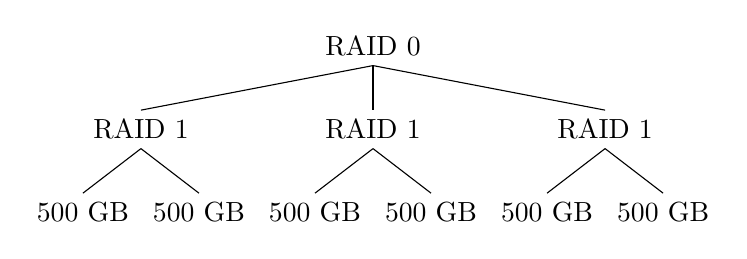
\begin{tikzpicture}
    \Tree
    [.RAID~0
        [.RAID~1
            [.500~GB ]
            [.500~GB ]
        ]
        [.RAID~1
            [.500~GB ]
            [.500~GB ]
        ]
        [.RAID~1
            [.500~GB ]
            [.500~GB ]
        ]
    ]
    \end{tikzpicture}
    \end{center}

    \begin{itemize}
        \item Ten system może przetwać równoczesną awarię \textbf{do trzech}
              dysków.\\

        \item \textbf{CECHY}
        \begin{itemize}
            \item \textbf{Najszybszy zapis i odczyt}.
            \item Odporność na błędy.
            \item Wykorzystuje efektywnie 50\% pojemności całkowitej.
            \item Najlepszy, ale najdroższy.
            \item Polecany w systemach baz danych, gdy
                  \textbf{liczba operacji zapisu}
                  jest \\większa niż 10\% liczby wszystkich operacji.
        \end{itemize}
    \end{itemize}

    \textbf{RAID 01 (0+1)}
    \begin{itemize}
        \item Różnice między RAID 0+1 i RAID 1+0 stanowi położenie każdego z
              systemów RAID.
        \item Jest uważany za \textbf{gorszy niż RAID 10}.
        \item \textbf{Nie przetrwa dwóch równoczensnych awarii}
              jeśli nie są to dyski z tego samego układu RAID.
        \item Po awarii jednego dysku, wszystkie dyski w drugim pasku stanowią
              krytyczne punkty. Połowa dysków przestaje być wykorzystywana.\\
              W systemie RAID 10 jeśli uszkodzeniu ulegnie jeden dysk, tylko
              jeden staje się krytycznym punktem układu.
    \end{itemize}

    \begin{center}
    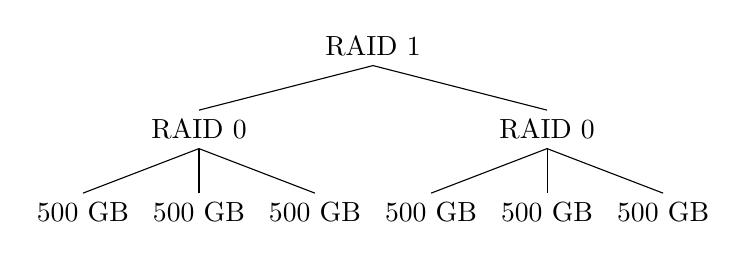
\begin{tikzpicture}
    \Tree
    [.RAID~1
        [.RAID~0
            [.500~GB ]
            [.500~GB ]
            [.500~GB ]
        ]
        [.RAID~0
            [.500~GB ]
            [.500~GB ]
            [.500~GB ]
        ]
    ]
    \end{tikzpicture}
    \end{center}

    \textbf{WAŻNE UWAGI}
    \begin{itemize}
        \item RAID nie powinien zastąpić odpowiedniej strategii robienia kopii
              zapasowych.
        \item Administrator musi wykonywać okresowo kopie zapasowe (pełne,
              różnicowe, plików, dziennika transakcji).
    \end{itemize}

    % section budowa_fizyczna_baz_danych_macierze_raid (end)

\pagebreak

    \section{Charakterystyka baz danych NoSQL} % (fold)
    \label{sec:charakterystyka_baz_danych_nosql}

    \horrule{0.5pt}
    Proszę \underline{powiedzieć co oznacza} termin skalowanie \textbf{poziome}
    w systemach baz danych i \textbf{jak realizowane jest} skalowanie poziome
    w bazach danych NoSQL.\\
    \horrule{0.5pt}

    \vskip 0.5cm

    \textbf{SKALOWANIE POZIOME}
    \begin{itemize}
        \item Jest to dodawanie dodatkowych "węzłów" do systemu, na przykład
              dodawanie nowego komputera do systemu.
    \end{itemize}

    \textbf{SKALOWANIE PIONOWE}
    \begin{itemize}
        \item Jest to dodawanie dodatkowych zasobów istniejącym "węzłom" w
        systemie, na przykład dodawanie RAM komputerowi w systemie.
    \end{itemize}

    \textbf{REALIZACJA SKALOWANIA POZIOMEGO}
    \begin{itemize}
        \item Rezygnacja z części funkcjonalności relacyjnych baz danych,
              brak relacji, transakcji, nie są zachowane własności ACID.
    \end{itemize}

    \horrule{0.5pt}
    Proszę \underline{podać główne typy} baz danych \textbf{NoSQL}.\\
    Proszę \underline{podać przykłady dokumentów} w formacie \textbf{JSON}.\\
    \underline{Jak} dokumenty są przechowywane w systemach \textbf{NoSQL}
    zawierających wiele węzłów (komputerów) połączonych siecią komputerową?\\
    Czy \underline{łączenie danych} z różnych dokumentów odbywa się na ogół w
    bazie danych
    (jak operacja \texttt{JOIN} w bazach relacyjnych), czy w aplikacji?\\
    Czy w bazach \textbf{dokumentowych} należy unikać redundancji tak, jak w
    systemach relacyjnych?\\
    \horrule{0.5pt}

    \vskip 0.5cm

    \textbf{GŁÓWNE TYPY}
    \begin{itemize}
        \item Klucz-Wartość
        \item Hierarchiczna struktura klucz-wartość
        \item Dokumentowe
        \item Grafowe
    \end{itemize}

\pagebreak

    \textbf{PRZYKŁAD JSON}
    \begin{minted}[mathescape,
               linenos,
               numbersep=5pt,
               gobble=2,
               frame=lines,
               framesep=2mm]{json}
   {
     "menu":
     {
       "id": "file",
       "value": "File",
       "popup":
       {
         "menuitem":
         [
           {"value": "New", "onclick": "CreateNewDoc()"},
           {"value": "Open", "onclick": "OpenDoc()"},
           {"value": "Close", "onclick": "CloseDoc()"}
         ]
       }
     }
   }
    \end{minted}

    \textbf{PRZECHOWYWANIE DOKUMENTÓW}
    \begin{itemize}
        \item Dokumenty rozrzucone po węzłach, każdy z węzłów czyta i zapisuje
              równolegle.
    \end{itemize}

    \textbf{ŁĄCZENIE DOKUMENTÓW}
    \begin{itemize}
        \item Odbywa sie w aplikacji.
    \end{itemize}

    \textbf{UNIKANIE REDUNDANCJI}
    \begin{itemize}
        \item Nie należy unikać redundancji.
        \item Liczy się szybkość dostępu do danych, często przez wielu
              użytkowników na raz.
    \end{itemize}

    % section charakterystyka_baz_danych_nosql (end)

    \newpage
    ~

\end{document}
